\section{Organisation} \label{Organisation}

L'organigramme visible en figure \ref{organigramme} ci-dessous présente les ressources humaines et leurs rôles principaux associés.

\begin{figure}[H]
   \centering
   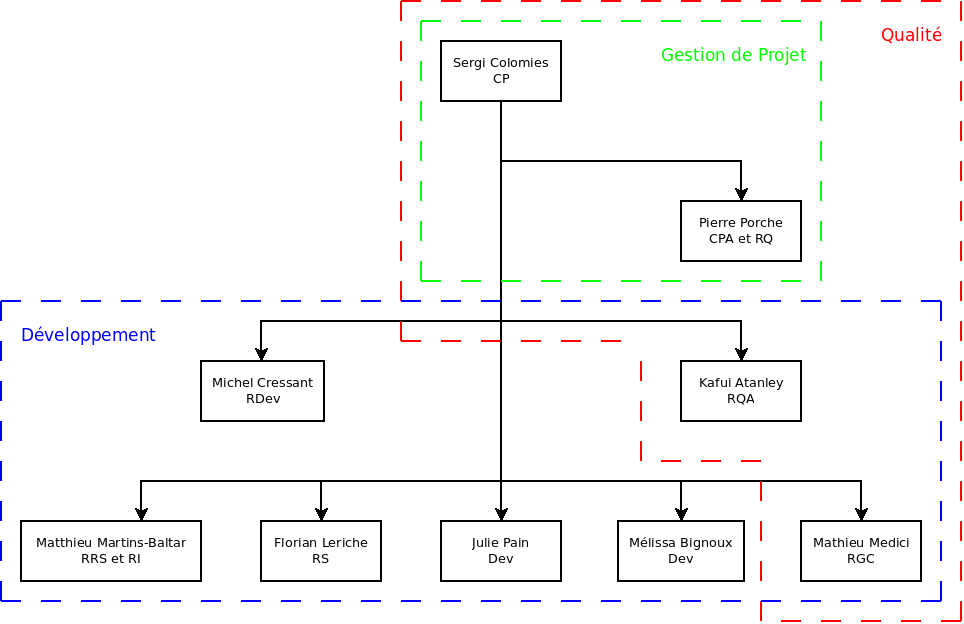
\includegraphics[width=15cm]{images/organigramme.png}
   \caption{\label{organigramme} Organigramme de \nomEquipe}
\end{figure}

\section{Compétences et formations} \label{CompetencesEtFormations}
\subsection{Rôles et compétences} \label{RolesEtCompetences}

\indent Chaque membre de l'équipe \nomEquipe{} est associé à un ou plusieurs rôles que l’on peut voir dans l’organigramme présenté ci-avant.\\

\indent Par défaut chaque membre possède le rôle de Développeur. On lui ajoute ensuite un rôle spécifique si nécessaire. Il pourra se voir attribuer le rôle de Pilote de Risque si celui-ci prend en charge la gestion d’un risque particulier.\\ 

\indent Le rôle de Responsable des Indicateurs sera également ajouté au Responsable Qualité, qui sera chargé de la mise à jour des indicateurs et du tableau de bord. \\

\indent Chaque attribution de rôle est justifiée par des compétences spécifiques que le titulaire doit posséder. C’est pourquoi les fiches de rôles spécifient les compétences requises pour effectuer une tâche. Ces fiches sont disponibles en annexe \ref{annexeFRo}. \\

\indent Ces Fiches de compétences, figurant dans le Dossier de Suivi de la Qualité, permettent de suivre le plan de formation de chaque membre de l’équipe PIC. Le formalisme d’une telle Fiche de compétences est disponible en annexe \ref{annexeFC}.\\

\indent Certaines personnes ont également des rôles plus particuliers détaillés dans la table \ref{repartRoles}. Chacun de ces rôles est défini dans une fiche de rôle disponible en annexe \ref{annexeFRo}.\\

\begin{table}[H]
\begin{tabular}[h]{|p{0.25\textwidth}|p{0.7\textwidth}|}
	\hline
	\rowcolor[gray]{0.85}
	Membre équipe PIC & Rôle(s) dans le projet \\\hline
	\Sergi &  \CP \\\hline
	\Pierre & \CPA, \RQ, \RI \\\hline
	\Kafui & \RQA, \D \\\hline
	\Mathieu & \RGC, \D \\\hline
	\Michel & \RD \\\hline
	\Matthieu & \RRS, \D \\\hline
	\Florian & \D \\\hline	
	\Julie & \D \\\hline
	\Melissa & \D \\\hline
\end{tabular}
\caption{\label{repartRoles} Répartition des rôles}
\end{table}

\subsection{Formations} \label{formation}

Si l'un des titulaires d'une tâche n'a pas les compétences requises pour la réaliser, il doit suivre une formation. Cette formation peut être organisée par un professeur, un autre membre de l'équipe PIC ou une personne externe. Si aucune de ces solutions n'est envisageable, le titulaire pourra s'autoformer.\\

Le temps nécessaire à une formation fait partie du planning du PIC et il apparaitra comme une tâche dans le planning. \\

Dans le cas où tous les membres du PIC devront s'autoformer à une technologie spécifique, deux membres du PIC devront réaliser un \QCM.

Un des deux \QCMCourt{} sera choisi pour que tous les membres du PIC soient évalués sauf le rédacteur de ce même \QCMCourt{} qui passera le second \QCMCourt.

Pour qu'une personne valide la formation, il faut que le \QCMCourt{} soit réussi à 66\% minimum. En cas d'échec à une évaluation, le membre devra se former de nouveau et repasser un \QCMCourt{} réalisé par un membre du PIC ayant obtenu cette compétence.

\section{Présence des membres}
\label{Présence des membres}

\subsection{Le temps de travail}
\label{temps_de_travail}
Selon le contrat d'étude, chaque membre de l'équipe doit faire un total de 24 heures de travail par semaine comprenant cinq jours ouvrés sur le PIC. Le Chef PIC et le Responsable Qualité possédant deux crédits de plus chacun, ils devront effectuer 27 heures par semaine comprenant cinq jours ouvrés. Si un ou quelques jours parmi ces cinq jours ouvrés sont fériés ou banalisés, on retire du volume horaire attendu les heures réservées à la réalisation du PIC sur ces jours fériés ou banalisés.

\subsection{En salle PIC}
\label{en_salle_pic}
Pour chaque membre, il est obligatoire de travailler minimum 18 heures en salle PIC par semaine comprenant cinq jours ouvrés. Pour le Chef PIC et le Responsable Qualité ce temps est de 20 heures par semaine comprenant cinq jours ouvrés. Si un ou quelques jours parmi ces cinq jours ouvrés sont fériés ou banalisés, on retire du volume horaire attendu les heures réservées à la réalisation du PIC sur ces jours fériés ou banalisés.\\

Un planning détaillé recensant les heures en salle de chaque membre sera créé et affiché.
Ce planning sera un moyen pour que le Chef PIC estime les ressources humaines disponibles à n'importe quel moment de la semaine.

\section{Locaux de réalisation du projet}
\label{Locaux de réalisation du projet}
\indent L'INSA, et plus précisément le département \ASI{}, met à disposition de chaque une salle de travail située dans le bâtiment Bougainville. Chaque équipe PIC bénificie de cette salle pour toute la durée du projet.
Concernant notre équipe, \nomEquipe, la salle qui nous a été attribué est ARC04.

\section{Inventaire du matériel mis à disposition}
\label{Inventaire du matériel mis à disposition}
Notre salle PIC a été fournie avec du matériel informatique dont l'inventaire est le suivant : \ref{annexeInventaire}.

\section{Inventaire des ressources informatiques}
\label{Inventaire des ressources informatiques}
Les ressources mises à disposition par le département \ASI{} pour l'équipe Unipik sont :

\begin{itemize}
	\item Un dépôt \git{} sur la plate-forme MonProjet de l'INSA Rouen;
	\item Un logiciel de gestion de projet PGPic.\\
\end{itemize}

Cependant il est possible que d'autres logiciels soient utilisés par l'équipe PIC tout au long du projet à condition que ceux-ci soient libres de droit d'utilisation.

\section{Matériel à acheter}
\label{Matériel à acheter}
\indent Aucun budget n'a été défini concernant le projet, l'application doit etre le plus proche possible de la gratuité (utilisation de logiciels et technologies issus du monde libre). \\
\indent Le secrétariat du département tient à jour un tableur où sont stockés les suivis de budget de toutes les équipes PIC.

\section{Eventuelle licence informatique à commander}
\label{Eventuelle licence informatique à commander}
\indent Pour le moment aucun achat de licence n'est nécessaire au projet.

\section{Matériel et/ou logiciel fournis par le client}
\label{Matériel et/ou logiciel fournis par le client}
\indent Pour le moment aucun prêt de matériel et/ou logiciel n'a été fait par le client.
\indent Dans le cas où des données seraient fournies à l’équipe PIC par le client, il faut faire un Procès-Verbal de réception à la récupération des données. A la fin du PIC, un Procès-Verbal de destruction des données doit être fait, pour certifier que les données ainsi que toutes les copies ont bien été détruites.

\section{Description des procédures relatives à l'écoute client}
\label{DescrProceduresRelativesALecouteClient}
\indent La communication avec le client devra s'effectuer à travers les documents de spécification interne et externe (\DSECourt , \DSICourt) (cf machin). Dans ces documents, les attentes du client seront prises en compte. Des réunions régulières devront également être réalisées ainsi qu'un \CRC{} après chaque réunion. Celui-ci devra être validé par le client afin d'éviter les incompréhensions entre les deux partis. \\
Les procédures à effectuer lors d'une réclamation ou une remarque du client devront être différenciées et sont décrites dans les parties suivantes.
   
\subsection{Remarques du client}
\label{RqClient}
A chaque remarque faite du client, une \FFT{} devra être réalisée (voir Annexe D \ref{fft}).

\subsection{Réclamations du client}
\label{ReclamClient}
A chaque réclamation du client, une \FFT{} (voir Annexe D \ref{fft})devra également être réalisée et un e-mail devra être envoyé au client. 

